\documentclass{llncs}
\usepackage{times}
\usepackage[T1]{fontenc}

% Comentar para not MAC Users
\usepackage[applemac]{inputenc}

\usepackage{a4}
%\usepackage[margin=3cm,nohead]{geometry}
\usepackage{epstopdf}
\usepackage{graphicx}
\usepackage{fancyvrb}
\usepackage{amsmath}
%\renewcommand{\baselinestretch}{1.5}

% CAPITAL LETTER LETTRINE
\usepackage{lettrine}

\begin{document}
\mainmatter
\title{Overview of Content-Delivery Networks Architecture}

\titlerunning{Paper Title}

\author{Afonso Silva\and Alfredo Gomes \and Axel Ferreira}

\authorrunning{Autor1 \and Autor2 \and Autor3}

\institute{University of Minho, Department of Informatics, 4710-057 Braga, Portugal\\
e-mail: \{a70387,a71655,a53064\}@alunos.uminho.pt
}

\date{\today}

\bibliographystyle{splncs}
%---------------- TITLE
\maketitle

%---------------- TABLE OF CONTENTS
%\tableofcontents
%\newpage

%%%%%%%%%%%%%%%%%%%%%%%%%%%%%%%%%%%%%%%%%%%%%%%%%%%%%%%%
%---------------- ABSTRACT							%()
%%%%%%%%%%%%%%%%%%%%%%%%%%%%%%%%%%%%%%%%%%%%%%%%%%%%%%%%
\begin{abstract}
Resumo...
\end{abstract}
%----------------
%%%%%%%%%%%%%%%%%%%%%%%%%%%%%%%%%%%%%%%%%%%%%%%%%%%%%%%%
\section{Introduction}									%(Axel)
%%%%%%%%%%%%%%%%%%%%%%%%%%%%%%%%%%%%%%%%%%%%%%%%%%%%%%%%

%\subsection{Context}
\lettrine[lines=2]{T}{he} Internet has its origins in the early 1980's and presented an exponential growth when commercial companies started to link to the existing academic and military networks during the 90's. As the popularity of the Internet increased the number of devices connected started to see an exponential growth.\\ 
% \subsection{Problems }
At that time networks were unreliable and internet communication protocols were designed in a robust fashion. As an example, Hypertext Transfer Protocol (HTTP) was designed to survive multiple packet losses and thus being a very chatty protocol, there are multiple Round-trip Time (RTTs) this causes a latency problem over long distance communication.
Modern networks are faster and more reliable, but most of the core protocols mentioned above don't take advantage of the increased reliability. %(Due to Backwards compatibility)
As the Internet role in daily life grew, new technologies star to emerge providing images videos and other dynamic content. This caused a bottleneck in servers with popular content.
The above problems, led to the development Content Delivery Networks.

%\subsection{What is a CDN?}
A Content Delivery Network (CDN) is a large network of distributed storage servers which cash the content in multiple locations strategically spread. Traditionally CDN servers are stored in ISP's facilities. This reduces both infrastructural costs to CDN Providers and ISP's costs by keeping popular content local, in contrast to bringing it from another ISP's network.

%\subsection{How does it Work?}
A CDN works by keeping a copy of the content in different locations. Whenever content is requested, management software calculates the best Server for accessing the content. This reduces distance to server which improves latency and minimizes packet loss. 
Since the calculations are dynamic, in case of a server malfunction another Server is chosen, providing redundancy.
%\subsection{CDN Service vs in House Solution}
Traditional CDN business model target bandwidth as a cost factor. This brings two advantages over a 'In House' solution:
First, there are no initial infrastructural costs, this is a big advantage. An example of the dimension of such structure's size would be Akamai's infrastructure. It is composed by more than 61,000 servers, spread across 1000 networks in 70 countries worldwide\cite{akamai};
Second, provides bandwidth on demand. In comparison with an 'In House' solution, there is no need to deal with both predictable and unpredictable traffic peaks.
Due to its large distributed infrastructure, and high bandwidth on demand CDNs are especially well suited to absorve a Denial of Service (DoS) attacks\cite{cdnetworks}.

%\subsection{Costs}
It is worth noting that CDNs bring cost per performance down. Despite that, CDNs are expensive, and currently are used mostly by big companies. It is imperative that CDN's get cheaper. This will allow more parties to use them, thus enhancing internet experience to the final consumer and reducing total internet traffic at the same time.
% Exemplo (�mbito de aplica��o) Netflix
An example of a service using a CDN (Amazon EC2) would be the popular movie streaming service Netflix.


\subsection{Purpose} %Prop�sito do paper
This paper's purpose is to provide organised information about different CDN architectures: the traditional large server infrastructure CDN, the Peer to Peer (P2P) CDN and a new trend of Hybrid architecture which relies on both Servers and Peers. 
	
%%%%%%%%%%%%%%%%%%%%%%%%%%%%%%%%%%%%%%%%%%%%%%%%%%%%%%%%
\section{Academic CDN (P2P)}							%(Afonso)
%%%%%%%%%%%%%%%%%%%%%%%%%%%%%%%%%%%%%%%%%%%%%%%%%%%%%%%%

\subsection{intro}
\subsection{ambito de aplica��o}
\subsection{Desafios Associados}

Netflix FHD 5Mbit/seg
	   UHD 25Mbit/seg

What are the Advantages?
	
	




According to Table~\ref{tab:TabelaExemplo}...


%%%%%%%%%%%%%%%%%%%%%%%%%%%%%%%%%%%%%%%%%%%%%%%%%%%%%%%%
\section{Hybrid CDN Architecture}								%(Alfredo)
%%%%%%%%%%%%%%%%%%%%%%%%%%%%%%%%%%%%%%%%%%%%%%%%%%%%%%%%

\subsection{intro}
\subsection{ambito de aplica��o}
\subsection{Desafios Associados}



\if		
	{What are the Disadvantages?}
	% Provider End (CDN Proviedr)
	% Client End (Content Provider)
	
\fi

\if
	Arquiteturas Propostas
		CDN Comercial (Uses CDN Servers at ISPs to provide content)
		CDN P2P Academic (Uses Both Dedicated Servers and Peer-user-owned Computers)
		(Hybrid) DCDN [Distributed CDN]
		-justifica��o- baixa de pre�os e acess�vel a + gente com 
\fi 

%%%%%%%%%%%%%%%%%%%%%%%%%%%%%%%%%%%%%%%%%%%%%%%%%%%%%%%%
\section{Lista de projetos atuais}							%()
%%%%%%%%%%%%%%%%%%%%%%%%%%%%%%%%%%%%%%%%%%%%%%%%%%%%%%%%	

The following list contains the most popular CDN service providers. According to \cite{reuters}, Akamai, being the biggest CDN provider, and is responsible for as much as 15\%-30\% of the internet traffic.

Another interesting perspective is to evaluate the offerings available. Most of them are commercial CDNs. 


-O paper "Standard IPTV CDN Architecture Interfaces" Fala sobre desafios
		� Falta de standards
		� Incompatibilidade entre as CDNs existentes (impossibilita a mobilidade)
		%-Lack of standards and Norms => hard to change provider

	
\if
	Cloud Content Delivery Networks
	
		Free CDNs
			BootStrap CDN\\
			CloudFlare\\
			CCDN\\
			Incapsula\\
			\dots\\
		Telco CDN\\
			AT\&T\\
			Verizon\\
			\dots\\
		Traditional CDNs\\
			Akamai\\
				Amazon\\
			Windows Azure\\
			HP Cloud\\
			CloudFlair\\
			\dots 

		Commercial CDN P2P\\
			BitTorrent\\
			Internap\\
			\dots\\
\fi


\section{Conclusion and Future Work}

nossa perspetiva
-Arquitectura h�brida 

- a contribui��o �nica � o paper focado nos custos gerais em fun��o das diferentes arquiteturas

-Referir que este paper est� limitado � perspetiva da bibliografia


%%%%%%%%%%%%%%%%%%%%%%%%%%%%%%%%%%%%%%%%%%%%%%%%%%%%%%%% 
%--------------- G L O S S A R I O ----------------%
%%%%%%%%%%%%%%%%%%%%%%%%%%%%%%%%%%%%%%%%%%%%%%%%%%%%%%%%
\if
	CDN - Content-delivery Network
	DCDN - Distributed Content-delivery Network
	DNS - Domain Name System
	RTT - round-trip time
	PoP - Points of Presence
	ASP - Application Service Provider
	SaaS - Software as a Service
	Caching -
	Mirroring -
\fi	
%%%%%%%%%%%%%%%%%%%%%%%%%%%%%%%%%%%%%%%%%%%%%%%%%%%%%%%%
%----------- B I B L I O G R A F I A -------------%
%%%%%%%%%%%%%%%%%%%%%%%%%%%%%%%%%%%%%%%%%%%%%%%%%%%%%%%%

% Inserir directamente os v�rios \bibitem 
\begin{thebibliography}{1}
\bibitem{reuters}
Anya George Tharakan, Subrat Patnaik: 
\newblock{"Strong dollar hurts Akamai's profit forecast, shares fall" (http://www.reuters.com/article/2015/04/28/us-akamai-tech-results-idUSKBN0NJ2IV20150428)}

\bibitem{akamai}
Erik Nygren, Ramesh K. Sitaraman, and Jennifer Sun.:
\newblock {"The Akamai Network: A Platform for High-Performance Internet Applications" (ACM SIGOPS Operating Systems Review, vol. 44, no. 3, July 2010)}

\bibitem{cdnetworks}
"How Content Delivery Networks Work" (http://www.cdnetworks.com/blog/how-content-delivery-networks-work/).
CDNetworks. Retrieved 22 September 2015.


% Exemplo de  um BibItem 
%	\bibitem{Nguyen99}
%	Nguyen, H., Walker, E.:
%	\newblock {First course in fuzzy logic}.
%	\newblock {Boca Raton: Chapman and Hall/CRC Press} (1999)
%	\end{thebibliography}


%%%%%%%%%%%%%%%%%%%% FIGURAS %%%%%%%%%%%%%%%%%%%%%%%%%%%
\if
De acordo com o ilustrado na Figura~\ref{fig:controller}
% Exemplo para inser��o de uma figura
\begin{figure}
\begin{center}
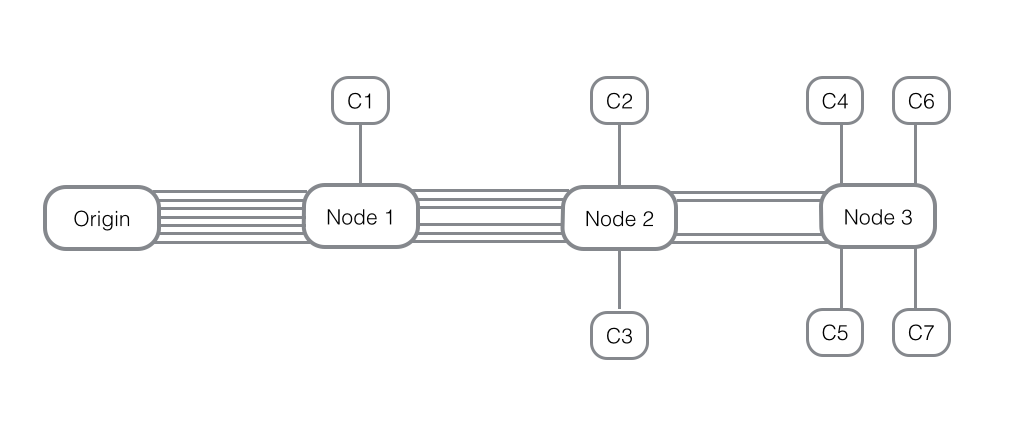
\includegraphics[scale=0.30]{nocdn} 
\end{center}
\caption{\label{fig:controller}Architecture of the unified QoS metric fuzzy controller.}
\end{figure} 

De acordo com o ilustrado na Figura~\ref{fig:controller}
% Exemplo para inser��o de uma figura
\begin{figure}
\begin{center}
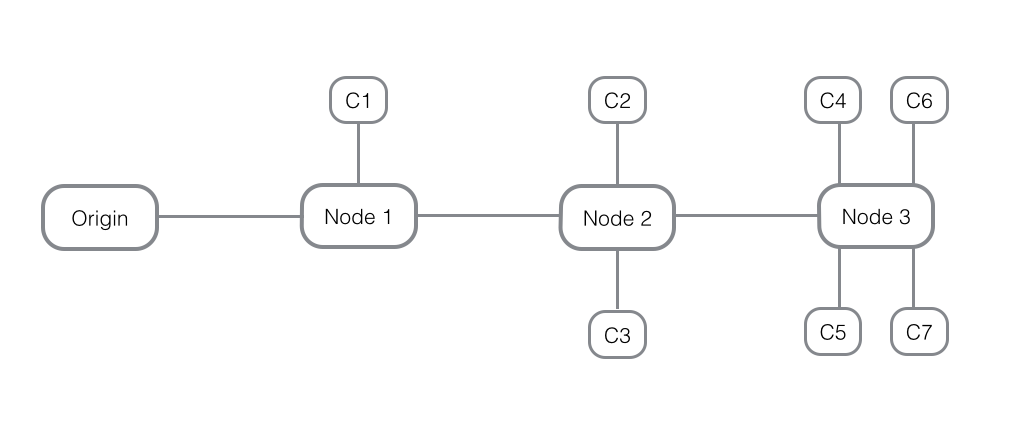
\includegraphics[scale=0.30]{cdn} 
\end{center}
\caption{\label{fig:controller}Architecture of the unified QoS metric fuzzy controller.}
\end{figure} 

De acordo com o ilustrado na Figura~\ref{fig:controller}
% Exemplo para inser��o de uma figura
\begin{figure}
\begin{center}
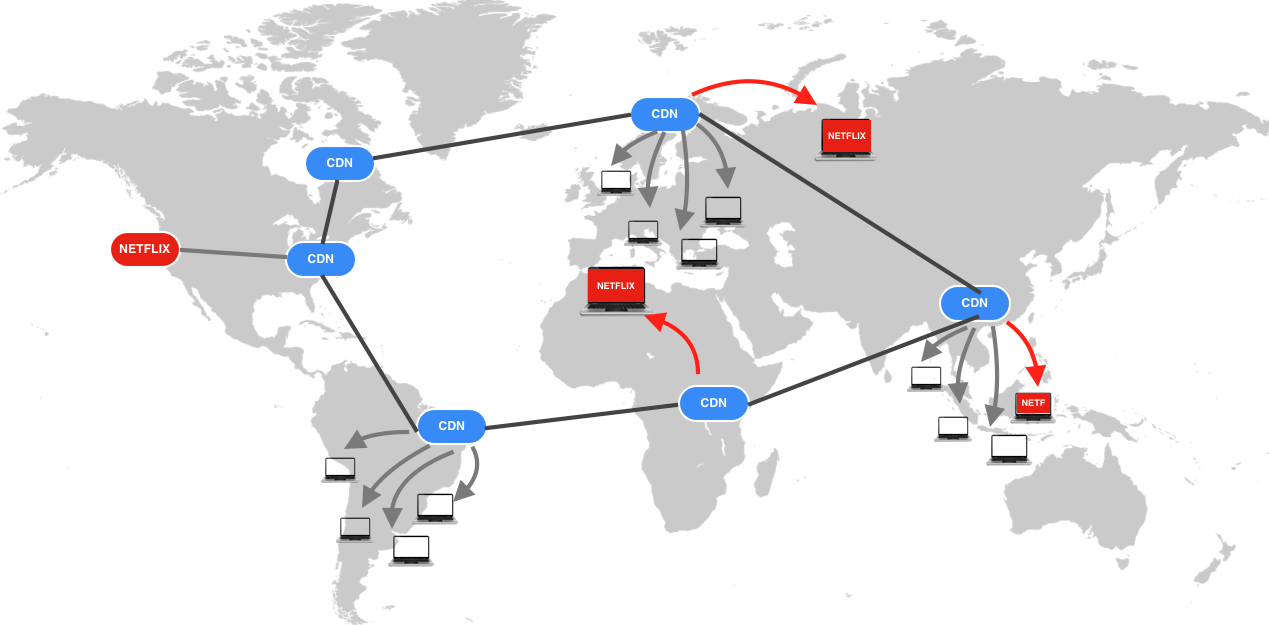
\includegraphics[scale=0.30]{map} 
\end{center}
\caption{\label{fig:controller}Architecture of the unified QoS metric fuzzy controller.}
\end{figure} 
\fi


\end{document}